\documentclass[a4paper,11pt]{article}

\usepackage{fullpage}
\usepackage{color}
\usepackage{hyperref}
\usepackage{amsmath}
\usepackage{amssymb}
\usepackage{tikz}
\usepackage{tabularx}
\usepackage{booktabs}
\usepackage{amsmath}
\usepackage{multirow}
\usepackage{layouts}
\usepackage{array}
\usepackage{pgf}
\usepackage{tikz}
\usepackage{epstopdf}
\usepackage{amssymb}
\usepackage{graphics}
\usepackage{fancyhdr}
\usepackage{eucal}
\usepackage{ifthen}
\usepackage{ifpdf}
\usepackage{lmodern}
\usepackage{amsthm}
\usepackage{catoptions} % For \Autoref


\usetikzlibrary{positioning}

\hypersetup{
  colorlinks,%
    citecolor=black,%
    filecolor=black,%
    linkcolor=black,%
    urlcolor=mygreylink     % can put red here to visualize the links
}

\definecolor{hlcolor}{rgb}{1, 0, 0}
\definecolor{mygrey}{gray}{.85}
\definecolor{mygreylink}{gray}{.30}
\textheight=8.6in
\raggedbottom
\addtolength{\oddsidemargin}{-0.375in}
\addtolength{\evensidemargin}{0.375in}
\addtolength{\textwidth}{0.5in}
\addtolength{\topmargin}{-.375in}
\addtolength{\textheight}{0.75in}


\newcommand{\resheading}[1]{{\large \colorbox{mygrey}{\begin{minipage}{\textwidth}{\textbf{#1 \vphantom{p\^{E}}}}\end{minipage}}}}

\newcommand{\mywebheader}{
  \begin{tabular}{@{}p{5in}p{4in}}
  {\resheading{Assignment 2: Single Agent Learning}} & {\Large 5 October, 2012}\\\vspace{0.2cm}
  \end{tabular}}

\begin{document}


\begin{center}
{\LARGE \textbf{Autonomous Agents}}\\ [1em]
\end{center}
\mywebheader

\begin{center}
{\Large By:} \\ \vspace{0.1cm}
{\Large Paris Mavromoustakos} \\  \vspace{0.1cm}
{\Large Georgios Methenitis} \\ \vspace{0.1cm}
{\Large Marios Tzakris}
\end{center}

\section*{Introduction}
A mixture distribution is the probability distribution of a random variable whose values can be interpreted as being derived from an underlying set of random variables. In the above figure, it is shown that a \textbf{latent variable} z underlies between class C and data-point x, thus latent variable z controls which data-points belong to which mixture element.

\section*{Exercise 1}

First, we loaded the given data files \texttt{banana.mat}, and, \texttt{spiral.mat}, each one of them contains two-dimensional data points, represent two different classes. The training set, which we used in order to train our classifier consists of 75\% of data points from class A, appended to 75\% of data points from class B, while the test set contains the remaining 25\% of both classes A and B. Figure~\ref{fig1}, shows the 2-D representation of the two classes of data-points.

\begin{figure}[h!]
  \centering   
      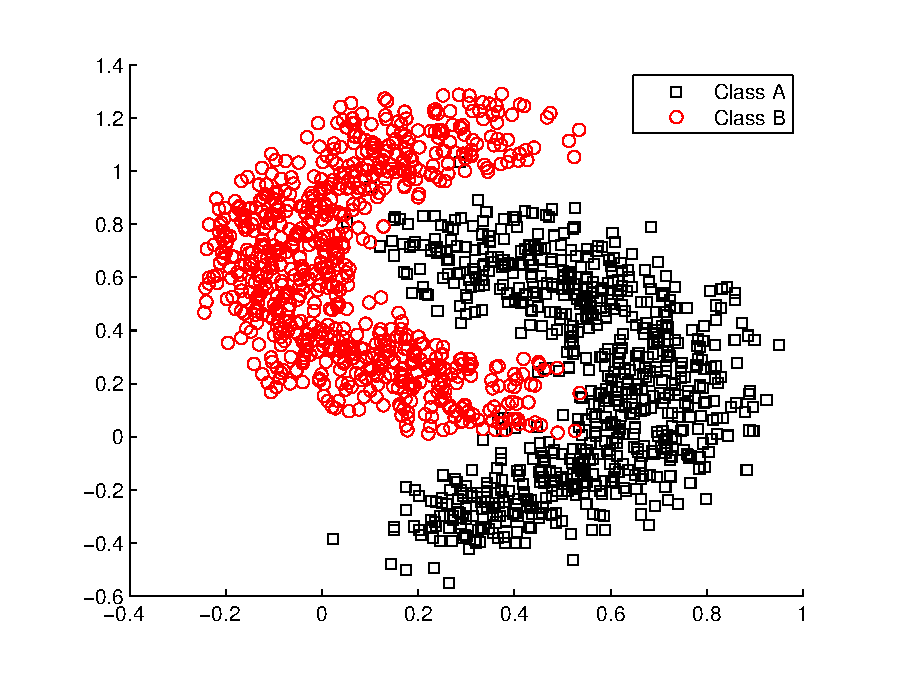
\includegraphics[width=0.49\textwidth]{figures/ABclasses.eps}\		
      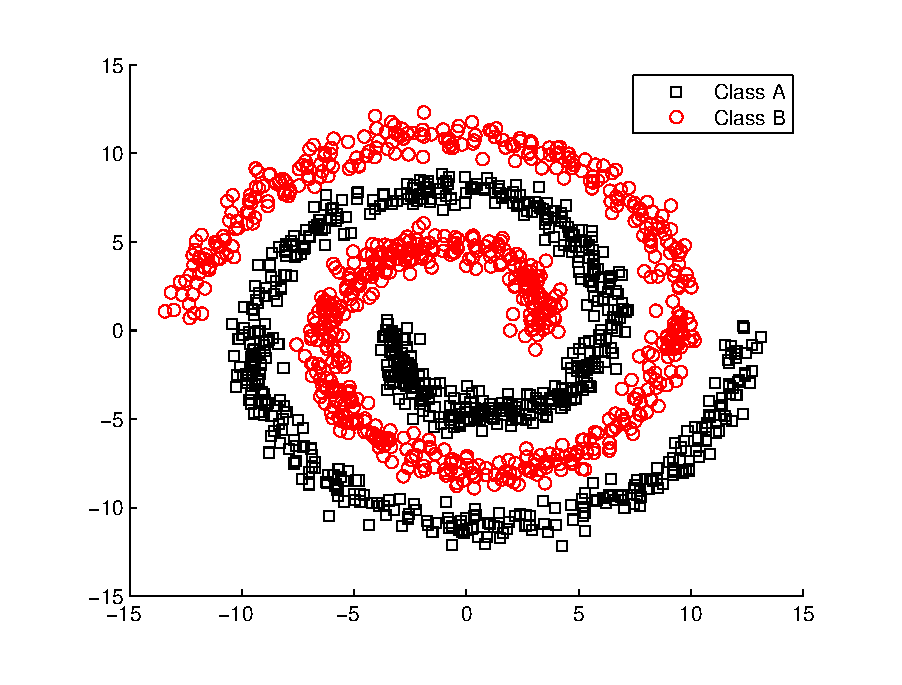
\includegraphics[width=0.49\textwidth]{figures/ABclassesSp.eps}
      
  \caption{Depiction of the 2-D data-points of the two given classes for the \texttt{banana.mat} (left) and \texttt{spiral.mat} (right).}
  \label{fig1}
\end{figure}

Looking into these data-points, we can figure out that the distribution of the data in both cases is following a "banana" and a spiral shape respectively. Therefore, a single 2-D Gaussian distribution could not be able to describe the class conditional probabilities well. For this reason, we do not expect the model to perform accurately. In order to perform the training, we need the prior probabilities, the mean $\mu_k$ of each class and the covariance matrix $\Sigma_k$  for each class $k \in \{A, B\}$. We set the prior probabilities $0.5$ as the number of the data for class A and B is the equal. Next, we can directly extract the mean and and the covariance for each class directly from the training data. The Matlab code for that is given below:\\

\begin{verbatim}
[A, B] = load( data_points )
TrainingSetA = A(1:length(A)*3/4,:)
TrainingSetB = B(1:length(B)*3/4,:)
TrainingSet = [TrainingSetA; TrainingSetB]

prior_probability_A = size(A,1)/(size(A,1)+size(B,1))
prior_probability_B = size(B,1)/(size(A,1)+size(B,1))

for i=1:size(TrainingSetA,1)
   sumAx = sumAx + TrainingSetA(i,1);
   sumAy = sumAy + TrainingSetA(i,2);
   sumBx = sumBx + TrainingSetB(i,1);
   sumBy = sumBy + TrainingSetB(i,2);
end

mean_A = [sumAx sumAy]/size(TrainingSetA,1);
mean_B = [sumBx sumBy]/size(TrainingSetA,1);

covariance_A = cov(TrainingSetA);
covariance_B = cov(TrainingSetB);

pA = mvnpdf(TestSet,mean_A,covariance_A);
pB = mvnpdf(TestSet,mean_B,covariance_B);

PostA = (pA .* prior_probability_A) ./ (pA .* pr_classA + pB .* pr_classB);
PostB = (pB .* prior_probability_B) ./ (pA .* pr_classA + pB .* pr_classB);
\end{verbatim} 
After the classification process we got the following confusion matrices and error rates for the our classifier:
\begin{description}
\item[Banana set]
\begin{align*}
Confusion\ Matrix &= 
\begin{bmatrix}
226 & 24 \\ 
26 & 224
\end{bmatrix},\\
error\ rate &= 0.1
\end{align*}
\item[Spiral set]
\begin{align*}
Confusion\ Matrix &= 
\begin{bmatrix}
174 & 76 \\ 
89 & 161
\end{bmatrix},\\
error\ rate &= 0.33
\end{align*}
\end{description}
As we said before, the way that we tried to perform classification in this type of data, did not perform well, mainly because, the shape of the data, and the fact that, data-points from the one class are located inside the other class, make it impossible for a simple 2-D Gaussian distribution to represent them.

\section*{Exercise 2}
To overcome the problem that we came across in the previous exercise, we had to use a different model that, the class-conditional distributions are modelled by a mixture of Gaussians distributions and not only by one as we did in the previous approach. 

Using the given function, \texttt{em\_mog(X,C,verbose)}, for the training set for both classes A and B, with input arguments the training set and then the number of mixture components we wanted to use. We followed this procedure for
both the training sets of classes A and B. Each iteration of the EM algorithm, calls two functions E-step and M-step.
E-step is responsible of updating the responsibilities for each $i$-component $ p(\textbf{z} | \textbf{t} , \bf{ \theta}^{old})$. For each component the update rule is:
\[
\gamma(z_{nk}) = \cfrac{\pi_k \mathcal{N}(\bf{x}_n | \bf{\mu}_k, \bf{\sum}_k)}{\sum_{j=1}^{K} \pi_j \mathcal{N}(\bf{x}_n | \bf{\mu}_j, \bf{\sum}_j)}
\]
The Matlab code for the E-step of the EM algorithm is the following:
\begin{verbatim}
L = length(MOG);
N = length(X(:,1));
Q = zeros(N, L);
total = zeros(N, 1);

for i = 1:L
    prob = MOG{i}.PI * mvnpdf(X, MOG{i}.MU, MOG{i}.SIGMA);
    Q(:,i) = prob;
    total = total + prob;
end

Q = Q ./ repmat(total, [1 L]);
LL = sum(log(total));
\end{verbatim}

Next, we had to implement the M-step of the algorithm. After the update of the responsibilities for each component, we have to re-estimate their parameters:
\begin{align*}
\pi_k^{new} &= \cfrac{N_k}{N}\	(1)\\
\mu_k^{new} &= \cfrac{1}{N_k} \sum_{n=1}^N \gamma(Z_{nk}) x_n\	(2)\\
\sum_k^{new} &= \cfrac{1}{N_k} \sum_{n=1}^N \gamma(Z_{nk}) (x_n - \mu_k^{new}) (x_n - \mu_k^{new})^T\	(3)
\end{align*}
The Matlab code for the M-step of the EM algorithm is the following:
\begin{verbatim}
L = length(MOG);
N = length(X(:,1));
    
for i = 1:L
        
   N_i = sum(Q(:,i));
   
   MOG{i}.PI = N_i / N; (1)
   MOG{i}.MU = sum(repmat(Q(:,i),[1 2]) .* X(:,1:2)) / N_i; (2)

   temp = (repmat(Q(:,i)', [2 1]) .* ((X(:,1:2) - repmat(MOG{i}.MU, [N 1]))') * (X(:,1:2)
           - repmat(MOG{i}.MU, [N 1]))); (3)
   
   temp = temp / N_i;
        
   if cond(temp) < 10^10
      MOG{i}.SIGMA = temp;
   end
end
\end{verbatim}
We also included a check in our M-step to avoid singularities. If c becomes larger than the number $10^{10}$, we do not perform the update. After these two steps of the EM algorithm, we check the convergence of the parameters. To realize when the algorithm converges, we just check how much change occurred in $\theta$ variable after the E-step.

\subsection*{``Banana'' data set}
As we expected, testing this classifier gave us better results than the one at the previous exercise. The number of components was an important factor on how the classifier would have performed. In Figure~\ref{fig23430comp}, you can see how the Gaussian components are formed throughout training process after the converge of the algorithm. 

\begin{figure}[h!]
  \centering   
      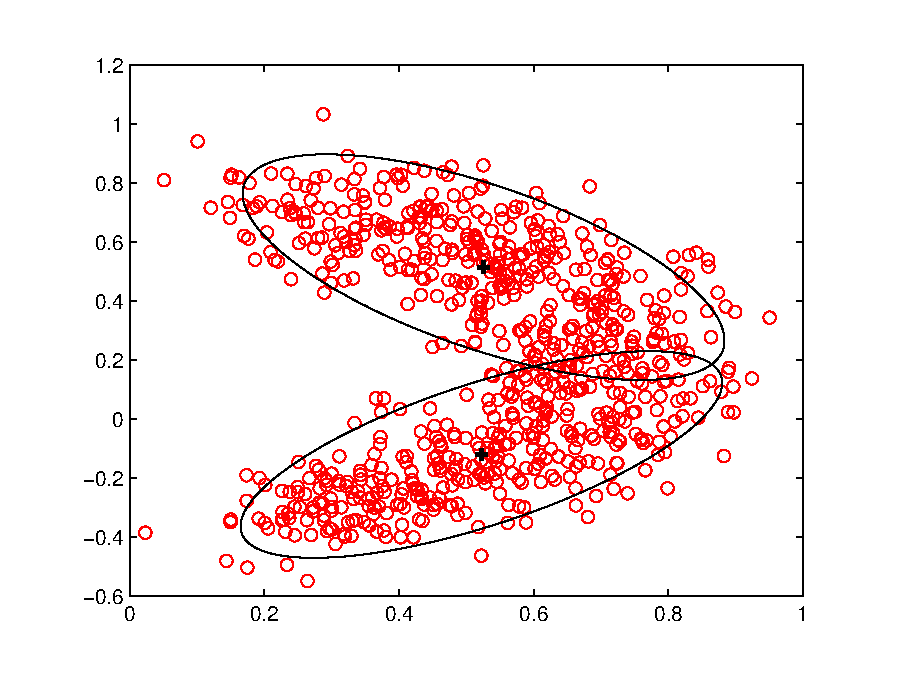
\includegraphics[width=0.35\textwidth]{figures/2comp.eps}\	
      \includegraphics[width=0.35\textwidth]{figures/3comp.eps}\	
      \includegraphics[width=0.35\textwidth]{figures/4comp.eps}\	
      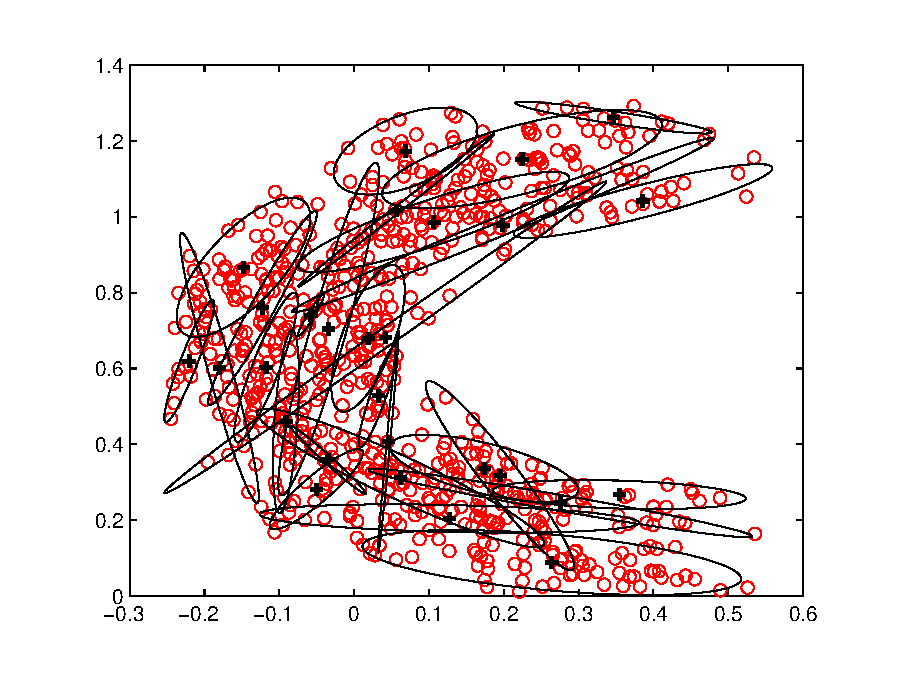
\includegraphics[width=0.35\textwidth]{figures/30comp.eps}    
  \caption{Illustration of the converged parameters, on the ``Banana'' dataset, using \textbf{2} (top-left), \textbf{3} (top-right), \textbf{4} (bottom-left) and, \textbf{30} (bottom-right).}
  \label{fig23430comp}
\end{figure}

In general, even in the training phase of our classifier we want to keep it  simple so the less components the fewer time it takes for the EM algorithm to converge. To test this, we performed a test using different number of components and evaluating the error rate. Figure~\ref{fig30comp}, presents the error rate in condition to the number of mixture components. Looking at this figure we can realize that the gain in the error rate, for 2 to 30 components, of our classifier is not big enough to convince us to use more than 2, 3, or 4 components. In contrary that the lower error rate was when we used 19 components, it took to the algorithm 650 iterations to converge for the training sets of both classes. In contrast, for only 3 components, algorithm needed 155 iterations. This big difference in the number of iterations led us to the conclusion that 4 is a good number of components for the ``banana'' set of data-points.


\begin{figure}[h!]
  \centering   
      \includegraphics[width=1\textwidth]{figures/1-30components.eps}      
  \caption{Error rate for EM algorithm using different number of componentson the ``Banana'' data.}
  \label{fig30comp}
\end{figure}

\subsection*{``Spiral'' data set}
\begin{figure}[b!]
  \centering   
      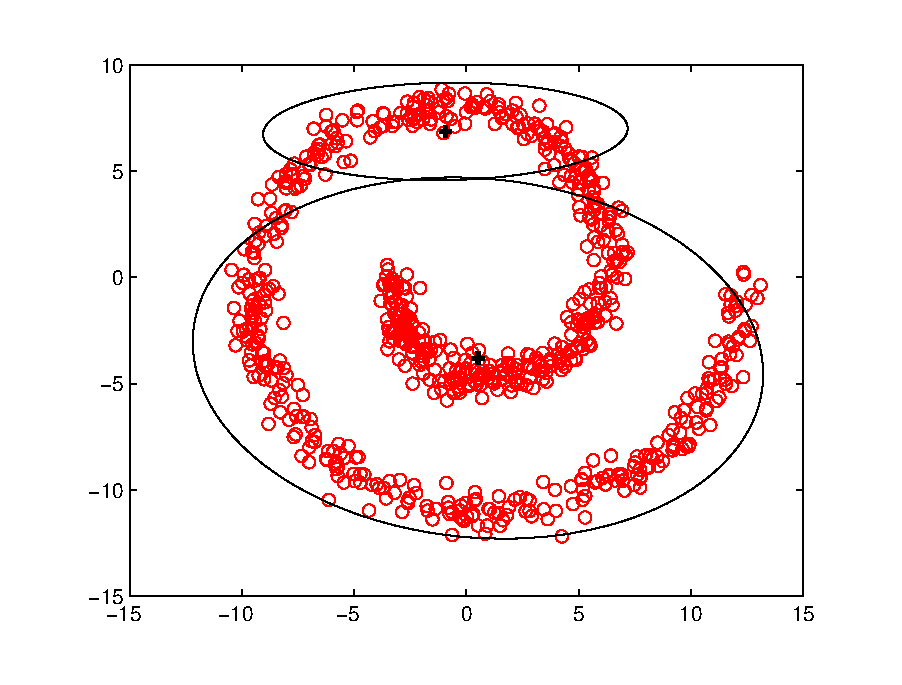
\includegraphics[width=0.35\textwidth]{figures/2compSp.eps}\	
      \includegraphics[width=0.35\textwidth]{figures/3compSp.eps}\	
      \includegraphics[width=0.35\textwidth]{figures/8compSp.eps}\	
      \includegraphics[width=0.35\textwidth]{figures/11compSp.eps}    
  \caption{Illustration of the converged parameters, on the ``Spiral'' dataset, using \textbf{2} (top-left), \textbf{3} (top-right), \textbf{8} (bottom-left) and, \textbf{11} (bottom-right).}
  \label{fig23430compSp}
\end{figure}
~
\begin{figure}[h!]
  \centering   
      \includegraphics[width=1\textwidth]{figures/30compSp.eps}      
  \caption{Error rate for EM algorithm using different number of componentson the ``Spiral'' data.}
  \label{fig30comp}
\end{figure}


As before, We train our classifier in the ``Spiral'' training set. In Figure~\ref{fig23430compSp}, you can see how the Gaussian components are formed after the converge of the algorithm. 



In contrary with the previous ``Banana'' dataset, after performing the same test as before using different number of components and evaluating the error rate on the ``Spiral'' dataset, we came up with different results. This happened due to the shape of the data, and the fact that the spiral shape cannot be represented by only two Gaussian distributions. We got appropriate, for a classifier, results after 7 we used more than 7 components. In fact, using 10 components gave us an error-free classifier, which shows the power of the EM algorithm especially in a such difficult dataset in which classes' data-points in not easy to be distinguished by other classifiers which we saw in previous labs or the first exercise of this lab.


\section*{Exercise 3}


\newpage
\section*{Conclusion}
\newpage


\end{document}

